\documentclass[11pt]{article}
\usepackage[margin=1in]{geometry}
\usepackage{graphicx}
\usepackage{booktabs}
\usepackage{amsmath}
\usepackage[hidelinks]{hyperref}
\usepackage{microtype}

\title{A Label-Free Runtime Safety Monitor for Frozen End-to-End Driving Planners,\\
Evaluated Closed-Loop at Benchmark Scale}
\author{Daniel Wahnich\\
\small Sentinel project --- \url{https://github.com/manfromnowhere143/sentinel}}
\date{July 2026}

\begin{document}
\maketitle

\begin{abstract}
End-to-end driving planners fail catastrophically in safety-critical closed-loop tests:
published NeuroNCAP results score UniAD at 1.84 out of 5, with collisions in 88--98\% of runs.
These collision failures are invisible to the open-loop displacement-error metrics that
dominate the field. We build a runtime monitor that reads only the frozen planner's own
outputs: its planned trajectory, the objects it detects, and their tracked motion. The monitor
uses no labels, no training, and no privileged simulator state. When it predicts a collision,
it commands a full stop, holds that stop, and returns control only after consecutive clear
frames confirm the threat has passed.

Across nineteen pre-registered campaign iterations and an independent verification pass we
show six results. (1) The published NeuroNCAP UniAD baseline reproduces: rerunning the full
benchmark at 20 runs per scenario yields a pooled score of 2.12 against the published 1.84. To
our knowledge, we are the first to independently reproduce this baseline; a concurrent rerun
by the DMAD authors (2.11), discussed in related work, corroborates the value. (2) The
monitor, a union of two label-free geometric detectors with the threat-cleared stop-and-release
policy, raises the full-benchmark score to \textbf{2.91} ($+0.783$, 95\% CI
$[+0.605, +0.928]$) while leaving behaviour in clean scenes, scenes with no staged threat,
identical to the unmonitored planner. Its cost on our deployment metric, which combines safety with driving
progress, is statistically indistinguishable from zero ($-0.03$, 95\% CI $[-0.13, +0.07]$).
(3) No softer intervention we tested could replace the committed stop. Three evasive
maneuvers, a calibrated crawl, and a geometric threat-router all failed their pre-registered
falsification criteria. The router failed narrowly, on a single misrouted crossing, while
showing that a monitor with a positive deployment effect is achievable ($+0.226$ vs.\ the
unmonitored planner, CI $[+0.004, +0.421]$). (4) An RSS-style formal safety envelope on
identical inputs achieves the campaign's best raw safety scores, but only by nearly refusing
to drive. This quantifies in closed loop the over-conservatism of formal envelopes that the
literature so far only asserts. (5) We locate why the planner cannot save itself. In
safety-critical frames, where a collision is imminent, the planner's candidate trajectories
collapse onto its dangerous main plan: UniAD's candidates span 14\,m of diversity on benign
frames (frames where the planner is not on a collision course) but only 4\,cm under imminent
collision, and VAD retains partial diversity that stays below a pre-registered viability bar.
A separately trained candidate generator that reads the frozen planner's internal planning
embeddings is accurate on benign frames, yet on the same dangerous frames it produces
\textbf{zero feasible escapes}, where a feasible escape is an alternative trajectory that is
both kinematically drivable and collision-free. The collapse therefore sits in the planner's
internal planning representation, not in any decoder above it. (6) Two independent failure
analyses, one on cross-planner transfer and one on intervention routing, converge on the same
bottleneck: the quality of the object tracking the monitor consumes.

One of our own earlier headline claims, that the monitor's deployment effect was net positive,
was withdrawn by our own audit after we found that deterministic episode replays had been
pooled as if they were independent samples; the claim was later re-established on genuinely
independent episodes. Six experiments whose pre-registered hypotheses failed are published in
full rather than discarded. All raw per-frame evidence is already released: it is committed in
the public repository, and every number in this paper regenerates from it.
\end{abstract}

\section{Introduction}
Open-loop planning metrics on nuScenes are saturated and gameable: an ego-state MLP with no
perception outperforms published end-to-end planners on displacement error
\cite{bevplanner}. Closed-loop evaluation under safety-critical perturbation tells the
opposite story: state-of-the-art planners collide in the vast majority of adversarial episodes
\cite{neuroncap}. Runtime assurance belongs in this gap. If a frozen planner's failures can be
predicted from its own outputs, a small monitor can intervene before they become collisions,
without retraining, fleet data, or privileged simulator state.

This paper reports a complete measurement campaign on that thesis. Its contributions are the
six numbered results in the abstract. Its method matters as much as its numbers: every
iteration of the campaign was pre-registered, with falsification criteria written down before
any data was collected; every comparison pairs the monitored and unmonitored arms on identical
episodes; every number can be regenerated from raw evidence committed in the public
repository; and the campaign's one statistical over-claim was caught by our own audit,
withdrawn, and re-established on fresh data.

\section{Related work}
\textbf{Runtime monitors for end-to-end planners.} CATPlan/RiskMonitor \cite{catplan} is the
canonical learned monitor: a transformer decoder trained on the sign of the planner's
collision loss, reading UniAD/VAD internal queries, paired with a braking policy (a 66.5\%
closed-loop collision-rate reduction on NeuroNCAP). Argus \cite{argus} attaches a takeover
fallback that generates its own replacement trajectory in CARLA. Centaur \cite{centaur}
adapts the planner's weights at test time. Our monitor differs on each axis. It uses
label-free geometry over the planner's own outputs, with no trained head. It never invents a
replacement trajectory; the failures of our evasion, crawl, and routing experiments
(\S\ref{sec:negI}) suggest this restraint is not merely simpler but structurally safer. It
performs no weight updates. And it is validated with a progress-aware metric that none of the
above report.

\textbf{Retrained planners on the same benchmark.} Concurrent work improves NeuroNCAP scores
by retraining or replacing the planner rather than monitoring it: BridgeAD \cite{bridgead}
reports 2.98--3.06 under the same trajectory post-processing protocol in which UniAD scores
1.84, and a VLM-agent system reports 3.49 in the protocol without post-processing
\cite{imagidrive}. Those results are complementary rather than comparable to ours: they change
the planner, while this campaign measures what a training-free monitor buys on the planner
exactly as shipped. Independently, DMAD's own rerun of the UniAD baseline (pooled 2.11)
\cite{dmad} corroborates the reproduction reported here (2.12).

\textbf{Runtime selection among a frozen planner's candidates.} Scoring and re-ranking a
planner's candidate trajectories is an active paradigm \cite{diver,gtrs,diffusiondrive}, but
in every instance we could verify, the scorer is co-trained within the planner's own pipeline
and evaluated on the non-reactive NAVSIM benchmark. We found no published work that re-ranks a
\emph{frozen} planner's native candidates at runtime using an external safety signal. Our
measurements close this mechanism for the planner's command-indexed candidates, which collapse
precisely when they are needed (\S\ref{sec:negII}), and reopen it for separately trained
candidate generators.

\textbf{Mode collapse under threat} is documented as a training-time phenomenon
\cite{awta}, with explicit metrics reported only for trajectory prediction
\cite{modecollapse}. To our knowledge, our measurements of candidate diversity conditioned on
imminent collision, taken closed-loop on two planners' own candidate sets, are the first of
their kind. Likewise, we found no prior closed-loop report of deployment-aware statistics for
a runtime monitor (combined progress-and-safety scores with bootstrap confidence intervals,
intervention budgets, detection lead time), and no prior closed-loop quantification of how
over-conservative a formal safety envelope \cite{rss} is in practice.

\section{Apparatus and methodology}\label{sec:apparatus}
The apparatus is three public containers on one L4 GPU: the NeuroNCAP orchestrator, which
drives the scenario actor and scores each episode; the NeuRAD neural renderer, which produces
photoreal multi-camera frames from real nuScenes drives; and the frozen planner, which serves
\texttt{/infer} and carries the monitor as a $\sim$150-line patch that an environment variable
enables or disables per experimental arm.

NeuroNCAP episodes replay deterministically for a given run index. We established this
property mid-campaign. It first invalidated an early pooled claim (\S\ref{sec:verif}), and it
then strengthened the design: because both arms replay the identical episode at the same run
index, every comparison in this paper is a paired comparison on identical episodes. We call
such comparisons \emph{seed-paired}. The determinism is verified at scale: the first six run
indices of the 20-run measurement reproduce the earlier 6-run measurement exactly, on every
scenario pair, in both arms.

The same methodology held for all nineteen iterations of the campaign. Hypotheses and
falsification criteria were frozen in writing before data collection. Every reported delta
carries a seed-paired bootstrap confidence interval. Per-frame monitor decision logs, per-run
trajectories, and run logs are committed for every arm. Experiments whose pre-registered
hypotheses failed are published with the same weight as those that succeeded.

\section{The monitor}
The monitor brakes when either of two conditions holds: the closest approach between the
planner's intended path and a tracked object's path falls below 1.5\,m, or the observed
time-to-collision with a closing agent falls below 2.5\,s. The two conditions catch physically
distinct failure modes. The first catches side crossings, where the planned path and an
object's path genuinely intersect. The second catches the head-on approach that the planner's
own optimism hides: on runs that end in collision, the planner's plan claims 3--4\,m of
clearance. Object velocity is \emph{observed}, by ego-motion-compensated tracking of each
object under a persistent identity, rather than taken from the planner's motion forecast; the
forecast is optimistic on exactly the runs that collide. The underlying signal is real and
cheap: the planner's own outputs predict its collisions with an AUROC of 0.83.

When the monitor triggers, the stop is \emph{latched}: the vehicle stays stopped even if the
trigger was spurious, which makes a false alarm safe. The latch \emph{releases}, returning
control to the planner, only after four consecutive frames verify that the planner's current
plan is clear of threats. We call this full configuration, the two detectors plus the
threat-cleared release, the \emph{released union}. Throughout the paper, \emph{safe-progress}
denotes our deployment metric: the product of episode safety and driving progress. The release
strictly dominates a latch that never releases: safety is identical, and safe-progress
improves by $+0.246$ (CI $[+0.206, +0.293]$).

\section{The benchmark result}
\begin{table}[h]\centering
\begin{tabular}{lrr}
\toprule
pooled, 14 official scenes ($n{=}20$/pair) & unmonitored UniAD & $+$ released union\\
\midrule
NeuroNCAP score (0--5) & 2.12 \;{\small(published 1.84)} & \textbf{2.91}\\
side collisions & 74\% & \textbf{44\%}\\
stationary collisions & 29\% & \textbf{18\%}\\
frontal (score / collisions) & 1.24 / 78\% & 1.78 / 90\%\\
safe-progress & 2.40 & 2.36\\
\bottomrule
\end{tabular}
\caption{The full-benchmark measurement: 799 episodes, seed-paired. Benchmark delta $+0.783$,
CI $[+0.605, +0.928]$; safe-progress delta $-0.03$, CI $[-0.13, +0.07]$.}
\end{table}

\begin{figure}[h]\centering
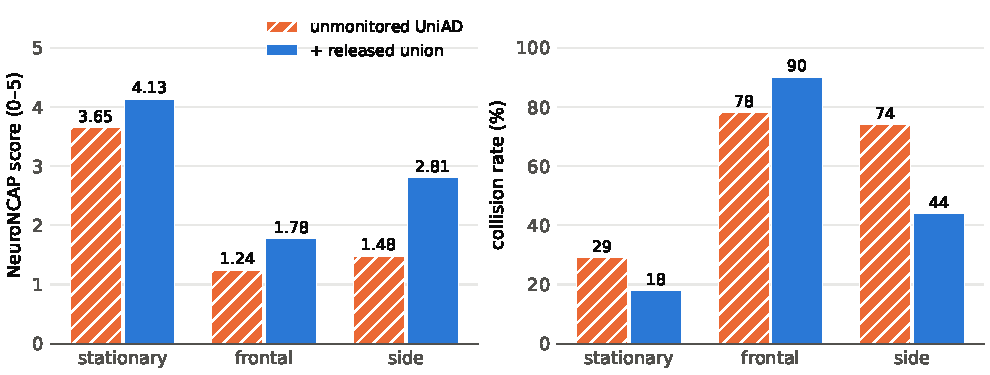
\includegraphics[width=\linewidth]{figures/fig1_benchmark.pdf}
\caption{Per-class results at $n{=}20$ runs per pair. In frontal scenarios the monitor
mitigates collisions rather than preventing them; the regression on the frontal 0346 scenario
is confirmed real and is reported as a named cost of the stop policy.}
\end{figure}

In the units a safety case uses, all computed from the committed decision logs: the median
detection lead is 2.5\,s before the moment of counterfactual contact, that is, before the
collision that occurs in the unmonitored arm (Fig.~\ref{fig:lead}); the monitor spends 11
brake frames per 242 benign meters driven; and the mean frontal impact speed drops from 13.9
to 6.7\,m/s.

\begin{figure}[h]\centering
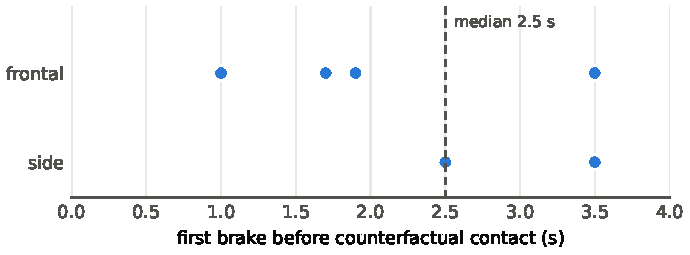
\includegraphics[width=0.8\linewidth]{figures/fig2_leadtime.pdf}
\caption{Detection lead time: the six lead-time events measurable under the strict contact
criterion, shown as individual events because six values are too few for a histogram.}
\label{fig:lead}
\end{figure}

\section{Negative results I: the stop is a position guarantee}\label{sec:negI}
Five designs that aimed to preserve more driving progress than the full stop were
pre-registered and refuted. The pattern of their failures is itself the finding.

Three evasive maneuvers fail under \emph{false} alarms: an evasive action taken on a spurious
trigger creates a crash where none was coming, and the third design crashes the benign scene
in 25\% of runs against the unmonitored planner's 10\%. A calibrated 2.0\,m/s crawl fails
under \emph{true} alarms: instead of halting short of a crossing object's path, as the stop
does, it delivers the ego vehicle into the crossing point, raising side collisions from 37\%
to 57\%. A geometric threat-router, which commands a stop when the projected object path
overlaps the planned corridor and a crawl otherwise (Fig.~\ref{fig:routing}), comes closest.
It records the campaign's first deployment-metric confidence interval excluding zero against
the unmonitored planner ($+0.226$, CI $[+0.004, +0.421]$), yet it still fails its
pre-registered safety gate on a single misrouted crossing.

The conclusion is twofold. First, the stop is not merely a speed reduction but a
\emph{position guarantee}: a stopped vehicle cannot be delivered into a collision point, so
the stop is safe whether the alarm is true or false, and it was the only tested intervention
with that property. Second, the router shows that a deployment-positive monitor is
demonstrably achievable, pending a routing signal that is safe on crossings
(\S\ref{sec:tracking}).

\begin{figure}[h]\centering
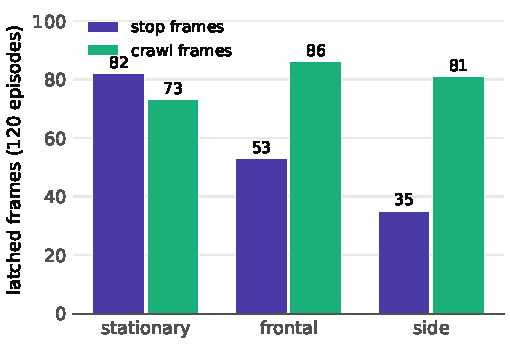
\includegraphics[width=0.55\linewidth]{figures/fig3_routing.pdf}
\caption{Frames in which the threat-router intervened, split by chosen action and scenario
class. The crawl frames account for the router's deployment gain; the misrouted side-class
crossing accounts for its safety failure.}
\label{fig:routing}
\end{figure}

\section{Negative results II: no plan B, envelope paralysis}\label{sec:negII}
\textbf{The planner has no plan B.} The natural escape from the stop's progress ceiling is to
execute a safer trajectory that the planner itself already proposes; such a takeover is safe
on false alarms by construction. Pre-registered checkpoints therefore measured whether a
low-risk candidate exists at the moments the executed plan is dangerous. It does not. UniAD's
command-conditioned candidates span 13.9\,m of diversity on benign frames and collapse to a
4\,cm spread under imminent collision (0 escapes in 37 dangerous frames). VAD's native modes
retain partial diversity (escapes in 21\% of those frames) but stay below the frozen 30\%
viability bar. We then trained the motivated successor: a 1.2M-parameter candidate head that
generates $K{=}8$ trajectories with an explicit diversity objective, conditioned on the frozen
planner's own planning-query embeddings and trained on 60 scenes disjoint from all evaluation.
The head is a faithful generator: on benign frames its best-of-$K$ error stays within its
pre-registered fidelity bar. Its repulsion term forces its candidates to diverge under threat.
And on the same 37 dangerous frames it yields \textbf{0 feasible escapes}: 16 diverging
candidates, every one violating kinematic limits. Three measurements by three routes agree.
The deficit is a property of the planning representation itself: under imminent collision,
that representation no longer contains a feasible alternative for any decoder to find.

\textbf{Stopping power is free; selectivity is not.} An RSS-style guaranteed-stopping
envelope, given inputs and an actuator identical to the monitor's, posts the campaign's best
raw safety (clean scenes 0\% collisions, frontal 30\%, side 0\%). It does so by driving
3.6--8.2\,m where the planner drives 21--32\,m, for a safe-progress of 0.88 against the
unmonitored planner's 1.83 (union minus RSS $= +1.345$, CI $[+0.944, +1.701]$).

\section{The binding constraint is tracking quality}\label{sec:tracking}
Two failure analyses, carried out from independent directions, converge on the same
constraint.

\emph{Transfer.} On a frozen VAD planner, the union prevents exactly the failures VAD has
(stationary collisions fall from 85\% to 0\%, side collisions from 65\% to 0\%) but brakes far
too often everywhere else. The decision logs attribute the over-braking to identity jitter:
VAD exposes no learned tracker, so nearest-neighbor association switches object identities
between frames, and each switch manufactures spurious closing speed.

\emph{Routing.} The router's single misrouted crossing traces to velocity dropout across
identity switches: when an object's identity changes, its velocity estimate momentarily
vanishes, and the projected-path test misses the crossing. All three named per-frame geometric
repairs were refuted offline on the committed logs: one is provably a no-op, one trades away
the mechanism it was meant to save, and one relies on a feature that does not separate unsafe
frames from safe ones.

In both analyses the discriminating signal is velocity continuity through identity switches, a
property of the tracking layer rather than of any decision rule built on top of it. An
association-and-filter layer built to this specification converts 12 of 13 unsafe crawl frames
in offline replay, yet fails its pre-registered every-frame bar by a single borderline frame
(0.2\,m). The gate held, and the layer never ran closed-loop. That result, together with the
caveat that offline replay may not perfectly reproduce closed-loop behaviour, is part of the
released record.

\section{Verification, reproducibility, and the incident record}\label{sec:verif}
An independent verification pass re-derived every claim from the raw evidence. It discovered
the episode determinism described in \S\ref{sec:apparatus}, and it found that an early pooled
validation had counted deterministic replays of the same episodes as independent replications.
We withdrew that headline claim and re-measured on genuinely unique episodes, where the claim
was re-established (mini-scene safe-progress $+0.398$, CI $[+0.133, +0.665]$).

The infrastructure incidents of the full-benchmark measurement are reported as part of the
measurement. Five machine-freezing events occurred across two physical hosts; an on-box vitals
instrument traced them to memory exhaustion on a swapless image. One scenario pair is reported
at $n{=}19$ because its final episode reproducibly froze the pre-swap host. No completed
episode was lost or re-measured differently; the exact reproduction of the earlier 6-run
measurement is the proof. Every number in this paper regenerates from raw evidence committed
in the public repository, using the commands in the repository README.

\section{Limitations}
This campaign uses one simulator (NeuroNCAP with the NeuRAD renderer), whose deterministic
replay we characterize and exploit; 20 runs per scenario pair against the published 100-run
protocol; and two planners. The VAD transfer result is bounded by the quality of the
identity-association layer. The RSS baseline implements the longitudinal form only. There is
no fleet data and no real-vehicle validation. Preventing frontal head-on collisions, as
opposed to mitigating them, remains open, and on this evidence it is not reachable by maneuver
invention from a label-free monitor.

\section{Conclusion}
A label-free monitor on a frozen planner lifts the full official NeuroNCAP benchmark from an
independently reproduced 2.12 to 2.91, with a confidence interval excluding zero, at a
deployment-metric cost statistically indistinguishable from zero. The campaign's negative
results carry as much weight as its wins: the stop's position guarantee, the planner's missing
plan B, the formal envelope's paralysis, the deployment-positive router that failed its safety
gate, and the convergence of two independent failure analyses on tracking quality. Together
they map the mechanism space for runtime driving assurance more sharply than the headline
number does, and they name the next constraint to remove.

\begin{thebibliography}{99}\small
\bibitem{neuroncap} Ljungbergh et al. NeuroNCAP: Photorealistic closed-loop safety testing for
autonomous driving. arXiv:2404.07762, 2024.
\bibitem{bevplanner} Li et al. Is ego status all you need for open-loop end-to-end autonomous
driving? arXiv:2312.03031, 2023.
\bibitem{bridgead} Zhang et al. Bridging past and future in end-to-end autonomous driving
(BridgeAD). CVPR 2025; arXiv:2503.14182.
\bibitem{dmad} Shen et al. Divide and merge: motion and semantic learning in end-to-end
autonomous driving (DMAD). arXiv:2502.07631, 2025.
\bibitem{imagidrive} ImagiDrive: driving-world-model imagination with a VLM agent. ICRA 2026;
arXiv:2508.11428.
\bibitem{catplan} CATPlan/RiskMonitor: collision prediction for end-to-end planners.
arXiv:2503.07425, 2025.
\bibitem{argus} Argus: runtime monitoring and takeover for end-to-end drivers. arXiv:2511.09032,
ASE 2025.
\bibitem{centaur} Centaur: test-time adaptation for robust planning. arXiv:2503.11650, 2025.
\bibitem{diver} DIVER: diversified trajectory generation. arXiv:2507.04049, 2025.
\bibitem{gtrs} GTRS: trajectory scoring at scale. arXiv:2506.06664, 2025.
\bibitem{diffusiondrive} DiffusionDrive. arXiv:2411.15139, 2024.
\bibitem{awta} Annealed winner-takes-all. arXiv:2409.11172, 2024.
\bibitem{modecollapse} Mode collapse happens: evaluating critical interactions in joint
trajectory prediction. arXiv:2506.23164, 2025.
\bibitem{rss} Shalev-Shwartz et al. On a formal model of safe and scalable self-driving cars.
arXiv:1708.06374, 2017.
\end{thebibliography}

\end{document}
